% !TeX encoding = UTF-8
\section{Постановка задачи}

Требуется разработать информационную систему для хранения и изменения объектов \texttt{Movie} и связанных с ними объектов \texttt{Coordinates}, \texttt{Person} и \texttt{Location}. Система должна создавать, показывать по идентификатору, редактировать и удалять фильмы в отдельных интерфейсах, выводить связанные данные и позволять выбирать ранее созданные вспомогательные объекты. Все изменения выполняются на сервере и сохраняются в PostgreSQL.

Главный экран должен показывать все предметные поля фильма в таблице с постраничной загрузкой, сортировкой и фильтрацией строковых значений по полному совпадению. Изменения одной сессии должны автоматически появляться у других авторизованных пользователей. Удаление объекта должно удалять зависящие от него объекты; некорректный ввод должен сопровождаться понятным сообщением.

Отдельный интерфейс должен поддерживать пять операций: удаление по сборам в США, расчёт среднего этого поля, поиск фильмов по начальному фрагменту \texttt{tagline}, перераспределение наград между жанрами и дополнительное награждение фильмов, длительность которых превышает порог. Эти действия реализуются в бизнес-логике приложения без хранимых процедур. Для приложения требуются управляемые компоненты Java EE и ORM-провайдер EclipseLink; ограничения предметной области должны соблюдаться как в ORM, так и в базе данных.

Основные поля и их ограничения приведены в таблице ниже.
\begingroup\small
% !TeX encoding = UTF-8
\begin{longtable}{L{3.5cm}L{3.2cm}L{7.8cm}}
\caption{Поля объектов и ограничения предметной области}\\
\toprule Поле & Тип & Ограничения\\\midrule\endfirsthead
\toprule Поле & Тип & Ограничения\\\midrule\endhead
\multicolumn{3}{l}{\textbf{Movie}}\\
id & Long & Не null; больше 0; уникальный; генерируется автоматически.\\
name & String & Не null; непустая строка.\\
coordinates & Coordinates & Не null.\\
creationDate & LocalDate & Не null; генерируется автоматически.\\
oscarsCount & int & Больше 0.\\
budget & long & Больше 0.\\
totalBoxOffice & Double & Может быть null; при наличии больше 0.\\
mpaaRating & MpaaRating & Не null.\\
director & Person & Может быть null.\\
screenwriter & Person & Дополнительные ограничения в задании не указаны.\\
operator & Person & Может быть null.\\
length & Integer & Не null; больше 0.\\
goldenPalmCount & Long & Может быть null; при наличии больше 0.\\
usaBoxOffice & int & Больше 0.\\
tagline & String & Не null.\\
genre & MovieGenre & Может быть null.\\\midrule
\multicolumn{3}{l}{\textbf{Coordinates}}\\
x & Integer & Не null; не больше 826.\\
y & Integer & Не null.\\\midrule
\multicolumn{3}{l}{\textbf{Person}}\\
name & String & Не null; непустая строка.\\
eyeColor & Color & Может быть null.\\
hairColor & Color & Может быть null.\\
location & Location & Может быть null.\\
birthday & ZonedDateTime & Не null.\\
height & Float & Может быть null; при наличии больше 0.\\
weight & Float & Может быть null; при наличии больше 0.\\
passportID & String & Не null; уникальный.\\\midrule
\multicolumn{3}{l}{\textbf{Location}}\\
x & Long & Не null.\\
y & Double & Не null.\\
name & String & Не null.\\\bottomrule
\end{longtable}
Допустимые значения перечислений приведены после UML-диаграммы классов. Поля вспомогательных объектов хранятся в PostgreSQL вместе с фильмами.

\endgroup

\section{Архитектура и модель данных}
\subsection{Компоненты приложения}

Серверное приложение собрано в WAR для Payara Micro. Компоненты Jakarta EE выполняют функции Java EE managed beans: REST-ресурсы и фильтр работают с HTTP-запросами, \texttt{MovieService} проверяет данные и реализует операции предметной области, \texttt{Database} создаёт \texttt{EntityManager} и управляет транзакциями. Зависимости внедряются через CDI. Браузер передаёт и показывает данные, не выполняя SQL-запросов и вычислений наград.

JPA-провайдером указан EclipseLink. В интеграционных тестах используется EclipseLink~4.0.5; внутри Payara приложение работает с предоставленной контейнером версией~4.0.1.payara-p3. Сущности, перечисления и конвертер временной зоны находятся в отдельном пакете. Диаграмма пакетов показывает направление зависимостей между частями приложения.

% !TeX encoding = UTF-8
\begin{figure}[H]
\centering
\begin{tikzpicture}[font=\small,pkg/.style={draw,align=center,minimum width=5.4cm,minimum height=1.45cm,fill=gray!5},dep/.style={dashed,-{Stealth},thick}]
\node[pkg] (ui) at (0,0) {\textit{«artifact»}\; webapp\\index.html, app.js, style.css};
\node[pkg] (web) at (0,-2.6) {\textit{«package»}\; web\\MovieResource, AuthResource\\AuthFilter, ErrorMapper};
\node[pkg] (svc) at (0,-5.4) {\textit{«package»}\; service\\MovieService, Problem};
\node[pkg] (repo) at (0,-8) {\textit{«package»}\; persistence\\Database};
\node[pkg,minimum width=4.4cm] (model) at (7,-5.4) {\textit{«package»}\; domain\\Movie, Person, Coordinates\\Location, AppState, enum\\конвертеры};
\node[pkg] (db) at (0,-10.6) {\textit{«database»}\; PostgreSQL\\movie, person, coordinates\\location, app\_state};
\draw[dep] (ui)--node[right]{HTTP / JSON} (web);
\draw[dep] (web)--node[right]{CDI @Inject} (svc);
\draw[dep] (svc)--node[right]{read / write} (repo);
\draw[dep] (repo)--node[right]{JPA / EclipseLink / JDBC} (db);
\draw[dep] (svc)--(model);
\draw[dep] (web.east) -| (model.north);
\draw[dep] (repo.east) -| (model.south);
\end{tikzpicture}
\caption{UML-диаграмма пакетов и внешних компонентов. Зависимости направлены от использующего компонента к используемому.}
\end{figure}


\subsection{Сущности и связи}

Фильм обязательно ссылается на координаты и может иметь режиссёра, сценариста и оператора. Каждый человек может ссылаться на место. Один вспомогательный объект допускается использовать для нескольких фильмов. Структуру и кратности связей показывает UML-диаграмма классов.

% !TeX encoding = UTF-8
\begin{figure}[H]
\centering
\begin{tikzpicture}[font=\scriptsize,box/.style={draw,rounded corners=1pt,align=left,inner sep=7pt,anchor=north west},link/.style={-{Stealth[length=2mm]},thick}]
\node[box,text width=6.0cm] (movie) at (0,0) {\textbf{\large Movie}\\\rule{6cm}{0.4pt}\\
id: Long \{identity\}\\
name: String\\
coordinates: Coordinates\\
creationDate: LocalDate \{DB default\}\\
oscarsCount: int\\budget: long\\totalBoxOffice: Double\\
mpaaRating: MpaaRating\\director: Person\\screenwriter: Person\\operator: Person\\length: Integer\\goldenPalmCount: Long\\usaBoxOffice: int\\tagline: String\\genre: MovieGenre\\\rule{6cm}{0.4pt}\\version: long \{optimistic lock\}};
\node[box,text width=5.6cm] (person) at (8,0) {\textbf{\large Person}\\\rule{5.6cm}{0.4pt}\\
id: Long \{identity\}\\name: String\\eyeColor: Color\\hairColor: Color\\location: Location\\birthday: ZonedDateTime\\height: Float\\weight: Float\\passportID: String \{unique\}\\version: long};
\node[box,text width=5.6cm,below=1.4cm of person.south west,anchor=north west] (location) {\textbf{\large Location}\\\rule{5.6cm}{0.4pt}\\id: Long \{identity\}\\x: Long\\y: Double\\name: String\\version: long};
\node[box,text width=6cm,below=1.0cm of movie.south west,anchor=north west] (coordinates) {\textbf{\large Coordinates}\\\rule{6cm}{0.4pt}\\id: Long \{identity\}\\x: Integer \{x $\leq$ 826\}\\y: Integer\\version: long};
\draw[link] (movie.east |- person.center) -- node[above,align=center]{3 роли} node[below]{0..* : 0..1} (person.west);
\draw[link] (person.south) -- node[right]{0..* : 0..1} (location.north);
\draw[link] (movie.south) -- node[right]{0..* : 1} (coordinates.north);
\end{tikzpicture}
\caption{UML-диаграмма сущностей. Стрелки показывают навигацию; каскад удаления направлен от справочного объекта к зависимым объектам.}
\end{figure}
\noindent Перечисления: \texttt{MpaaRating \{G, PG, PG\_13, R, NC\_17\}}, \texttt{MovieGenre \{WESTERN, COMEDY, TRAGEDY, HORROR\}}, \texttt{Color \{GREEN, BLACK, ORANGE, WHITE, BROWN\}}. Тип \texttt{Country \{GERMANY, VATICAN, ITALY, NORTH\_KOREA\}} включён в исходники, но не имеет связей в модели варианта.


Идентификаторы формируются в PostgreSQL посредством \texttt{IDENTITY}; дата создания фильма задаётся базой данных при вставке. В Java применяются \texttt{@NotNull}, \texttt{@Positive}, \texttt{@Max}, \texttt{@Enumerated} и связи \texttt{@ManyToOne}. В таблицах повторены обязательность, положительность, диапазон, уникальность паспорта и допустимые значения перечислений с помощью \texttt{NOT NULL}, \texttt{CHECK}, \texttt{UNIQUE} и внешних ключей. Поэтому прямой запрос к БД не позволяет обойти ограничения формы и сервиса.

Время рождения хранится как ISO-строка с часовым поясом через JPA-конвертер: при преобразовании в обычный \texttt{timestamptz} сохранился бы момент времени, но потерялось бы исходное имя зоны. Значения Java \texttt{Long} передаются в JSON десятичными строками, чтобы браузер не округлял большие целые числа. Для атрибутов, у которых задан лишь запрет \texttt{null}, пустая строка разрешена; дополнительные ограничения к исходным полям не добавлялись.

На кафедральном сервере приложение подключено к \texttt{pg:5432/studs}. В схеме учётной записи использованы отдельные префиксы для таблиц приложения и временных таблиц тестов. Таблицы, созданные ранее для других работ, при развёртывании не изменялись. Соответствие имён таблиц задаётся отдельными ORM-отображениями; локальный режим сохраняет обычные имена таблиц.

\subsection{Удаление и согласованность изменений}

Удаление координат или человека удаляет зависящие от них фильмы; удаление места удаляет связанных людей, а затем их фильмы. Сервис выполняет операции в этом порядке, а внешние ключи с \texttt{ON DELETE CASCADE} обеспечивают то же правило на уровне БД. Удаление одного фильма сохраняет вспомогательные объекты, которыми могут пользоваться другие фильмы.

Перед изменением данных транзакция блокирует служебную строку \texttt{AppState} для записи. Это последовательно выполняет групповые операции и защищает их от потери обновлений. У сущностей есть \texttt{@Version}; редактирование или удаление по устаревшей версии завершается ответом HTTP~409. Ревизия коллекции увеличивается вместе с изменением данных и откатывается при ошибке. Браузеры запрашивают ревизию раз в две секунды и при изменении обновляют представления, не стирая несохранённые поля открытой формы.

\section{Реализация интерфейса и запросов}

Меню разделяет фильмы, людей, координаты, места и специальные операции. Создание, просмотр, изменение и подтверждение удаления фильма открываются в отдельных диалогах. Форма позволяет выбрать существующие связанные объекты. В окне просмотра показаны и их атрибуты.

Таблица фильмов содержит отдельную колонку для каждого предметного поля. Постраничный запрос выполняется на сервере, сортировка дополняется идентификатором для устойчивого порядка. Имена полей сортировки и фильтрации проходят разрешённый список, а значения передаются параметрами JPQL. Фильтрация текстовых полей использует полное совпадение и учитывает регистр.

Авторизация использует HTTP-сессию с cookie \texttt{HttpOnly}; изменяющие запросы требуют CSRF-токен. При неверном значении поля сервер возвращает структурированную ошибку, которую форма показывает пользователю. Учебное приложение использует общую учётную запись без разделения ролей.

\begin{figure}[H]\centering
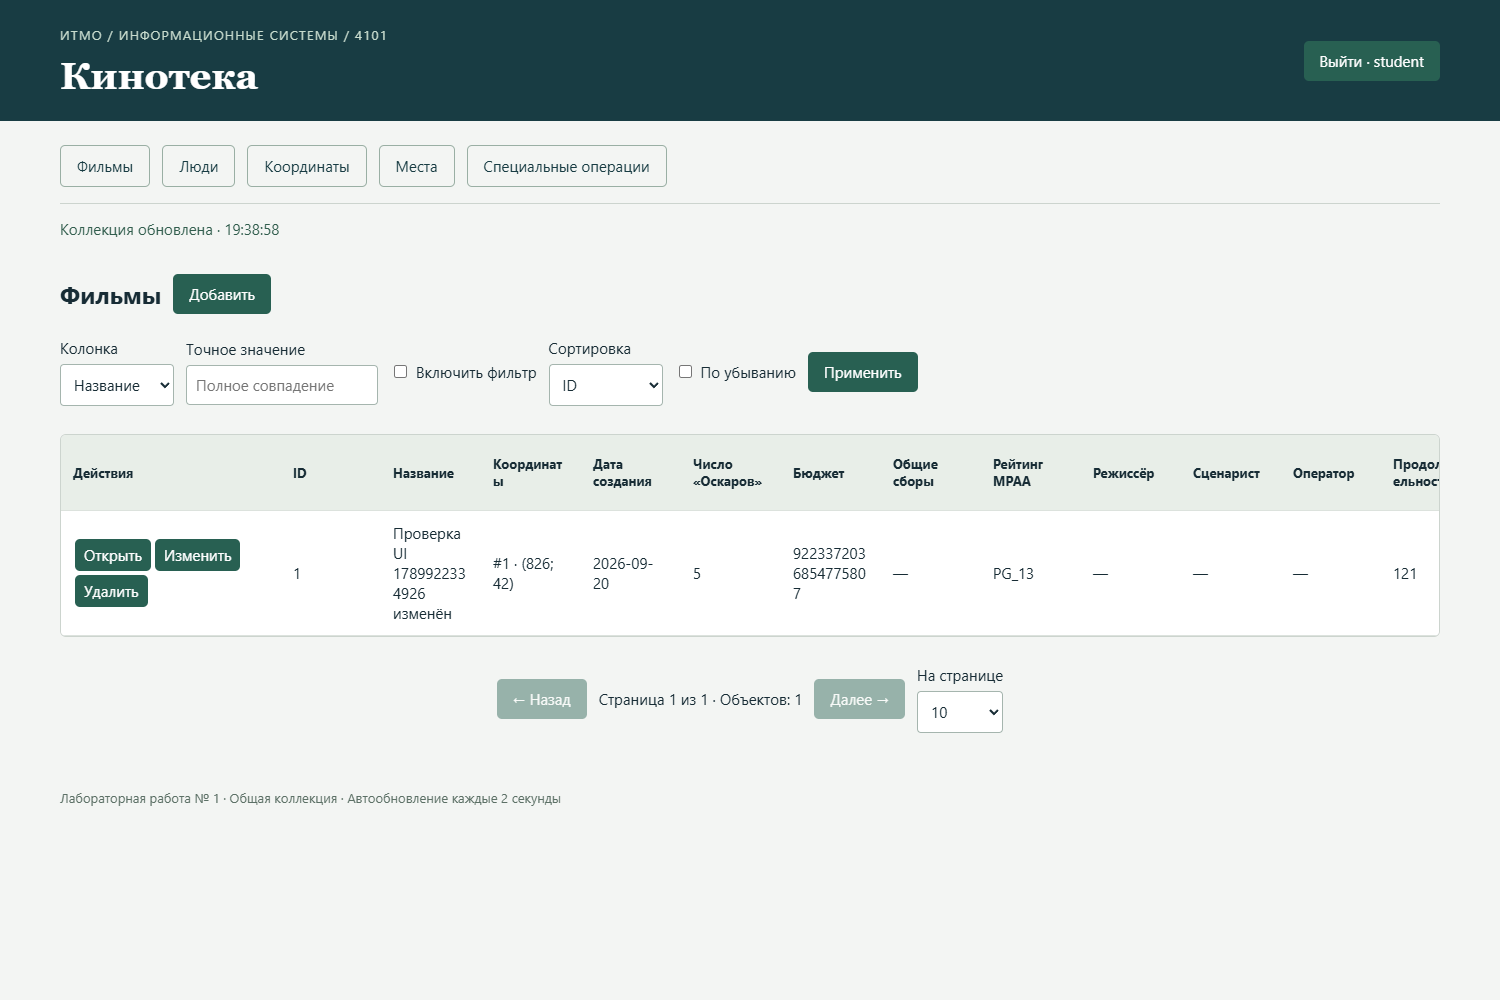
\includegraphics[width=\linewidth]{images/ui-table.png}
\caption{Таблица фильмов в работающем приложении; видна часть прокручиваемых колонок.}
\end{figure}

\begin{figure}[H]\centering
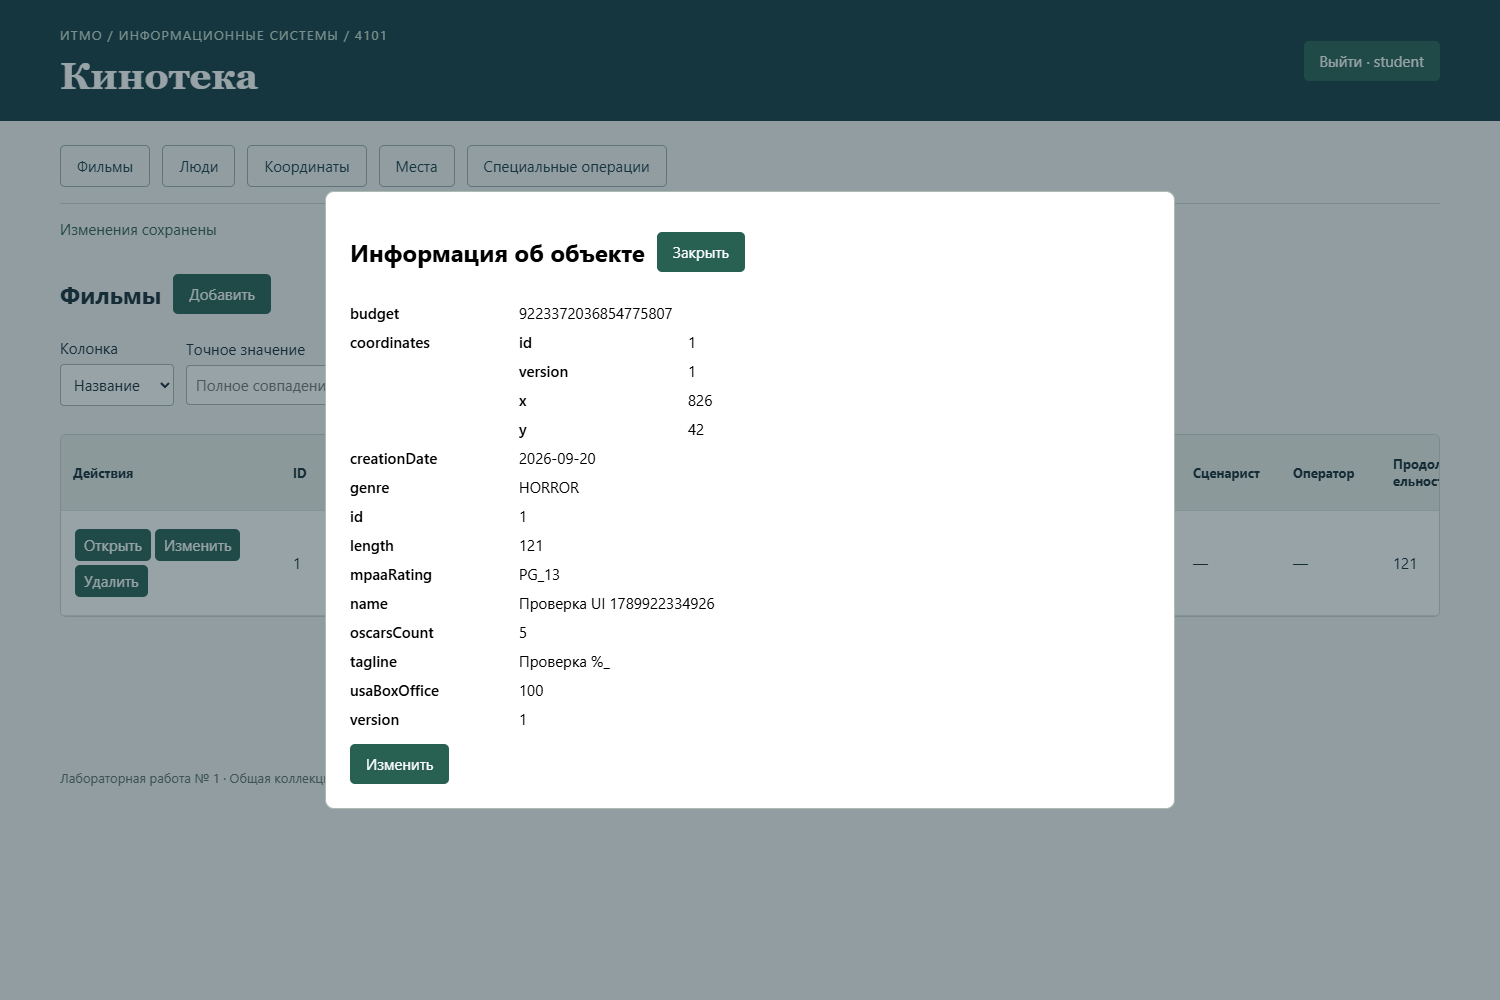
\includegraphics[width=0.88\linewidth]{images/ui-details.png}
\caption{Отдельное окно просмотра фильма и связанных координат.}
\end{figure}

\section{Специальные операции}

Удаление по \texttt{usaBoxOffice} выбирает фильмы с точно совпадающим значением и удаляет их в одной транзакции. Среднее вычисляется агрегатом JPQL \texttt{AVG}; для пустой коллекции возвращается \texttt{null}. Поиск по начальному фрагменту слогана использует \texttt{LIKE} с экранированием \texttt{\%}, \texttt{\_} и \texttt{!}, поэтому введённый фрагмент трактуется буквально. В отличие от него, фильтр главной таблицы требует полного совпадения.

У \texttt{oscarsCount} установлено обязательное условие $>0$. Поэтому при перераспределении каждый исходный фильм сохраняет одну награду, а остальные передаются фильмам целевого жанра. Для множества исходных фильмов $A$ и целевых фильмов $B$, где $n=|B|>0$, вычисляются
\[
S=\sum_{a\in A}\bigl(\operatorname{oscars}(a)-1\bigr),\qquad
q=\left\lfloor\frac{S}{n}\right\rfloor,\qquad r=S\bmod n.
\]
После присвоения каждому исходному фильму одной награды первые $r$ целевых фильмов по возрастанию ID получают по $q+1$ дополнительной награде, остальные --- по $q$. Общая сумма не меняется, а добавки отличаются максимум на единицу. Например, из исходных значений $(5,4)$ к целевым $(2,2)$ переносится $S=7$; итоговые значения $(1,1)$ и $(6,5)$ дают ту же общую сумму $13$. Если жанры совпадают или одна из групп пуста, операция отклоняется.

Дополнительное награждение затрагивает только фильмы с \texttt{length} строго больше порога. Перед записью проверяется переполнение целочисленного поля. Ошибка у любого фильма откатывает всю операцию, включая уже обработанные записи и ревизию коллекции.

\begin{figure}[H]\centering
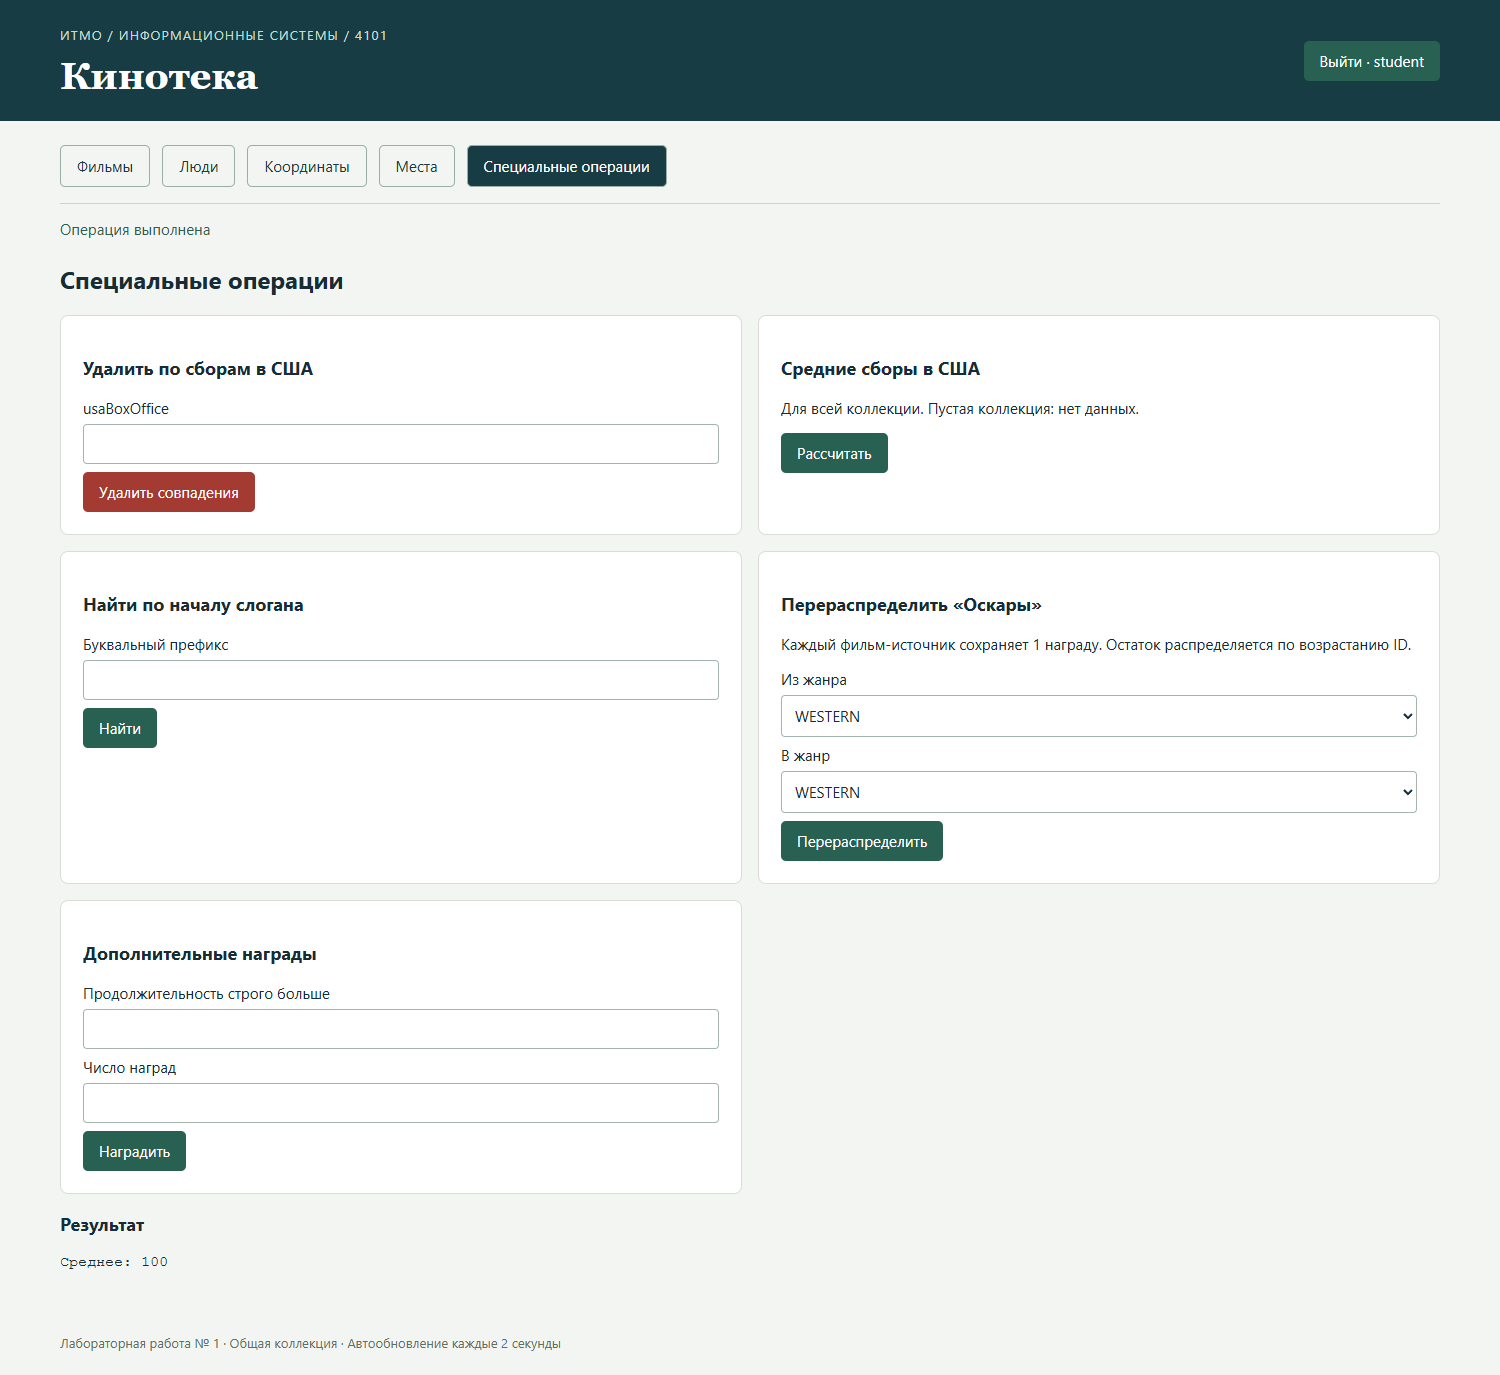
\includegraphics[width=0.82\linewidth]{images/ui-operations.png}
\caption{Отдельный экран специальных операций.}
\end{figure}

\section{Проверка работоспособности}

Реализация проверена на PostgreSQL с реальным JPA-провайдером, затем собрана и развёрнута на кафедральном сервере Helios под Java~21 и Payara Micro~6.2025.1. На этом сервере команда Maven \texttt{clean verify} завершилась успешно: \textbf{32 интеграционных теста, 0 ошибок, 0 неудач, 0 пропусков}. Тесты использовали отдельные временные таблицы той же PostgreSQL-базы; после завершения они были удалены. Ниже сгруппированы проверенные свойства.

\begin{longtable}{L{4.0cm}L{11.5cm}}
\caption{Основные группы интеграционных проверок}\\
\toprule Группа & Проверенное поведение\\\midrule\endfirsthead
\toprule Группа & Проверенное поведение\\\midrule\endhead
Создание и изменение & Генерация ID и даты, допустимые пустые и необязательные поля, сохранение идентичности, запрет изменения служебных полей.\\
Ограничения & Положительные значения, граница координаты, уникальность паспорта, допустимые перечисления, календарная дата и конечные числа; прямые SQL-попытки нарушения ограничений.\\
Чтение & Пагинация, сортировка, точный фильтр, обработка необязательных связей и передача максимального значения \texttt{long}.\\
Специальные операции & Среднее пустой и непустой коллекций, массовое удаление, буквальный префикс, остаток перераспределения и строгий порог длины.\\
Транзакции и связи & Откат при переполнении, конкурентные награждения без потерянных обновлений, обновление ревизии после фиксации, направленное каскадное удаление.\\
\bottomrule
\end{longtable}

Через SSH-туннель запущен сценарий Chrome и API против приложения на Helios. \textbf{Все 16 проверок прошли}: отказ неавторизованному запросу и неверному паролю, вход, CSRF, создание и валидация, просмотр связей, обновление и удаление, конфликт устаревшей формы, точная передача большого целого числа, работа специального интерфейса и автоматическое появление изменений во втором браузерном контексте. Ошибок JavaScript не обнаружено. Тестовые фильм и координаты после сценария удалены.

После остановки и повторного запуска Payara подтверждены ответ HTTP~200, работа авторизованного API и доступность пустой коллекции фильмов. Сервер слушает только локальный адрес; для просмотра применяется SSH-туннель. Работоспособность под промышленной нагрузкой не оценивалась.

\section{Исходный код проекта}

Исходные файлы приложения, SQL-схема и автоматические тесты составляют проект. Листинги кода в отчёт не включены.

\noindent\textbf{Ссылка на репозиторий GitHub:}\par
\noindent\url{https://github.com/utpwtb/ITMO/tree/main/5%20Information%20Systems/Lab/Lab1}

\section{Заключение}

Разработана информационная система управления фильмами и связанными объектами с хранением в PostgreSQL, JPA-отображением EclipseLink, управляемыми компонентами Jakarta EE и русскоязычным веб-интерфейсом. Реализованы операции создания, чтения, изменения и удаления, точная фильтрация, сортировка и пагинация, каскад зависимостей и пять специальных операций.

Согласованность изменений обеспечивается транзакциями, блокировкой групповых записей и проверкой версий. Взаимодействие двух пользователей подтверждено браузерным сценарием. Сборка и проверки на кафедральном сервере завершились успешно: 32 интеграционных теста и 16 проверок браузера и API. Принятое правило сохранения одной награды у каждого исходного фильма позволяет выполнить перераспределение без нарушения обязательного ограничения поля.
